\section{Unbalanced Tree Search}

The Unbalanced Tree Search benchmark (UTS) measures the rate of traversal of
a tree generated on the fly using a splittable random number
generator \cite{lcpc06}. Each node in the tree is identified by a 160-bit hash.
The UTS specification describes several cryptographic laws for computing the number and hashes of the children of a node.
The intend is to synthesize trees that are deterministic but unbalanced in unpredictable ways. 

A sequential implementation of UTS is straightforward. The code maintains a work list of pending nodes to visit, initialized with the root node of the tree. It repeatedly pops a node from the work list, computes the list of children for this node, and adds them to the work list, while keeping the count of the nodes processed so far. An empty work list signals the termination of the traversal.

In contrast, a parallel and distributed implementation of UTS is a challenge because of imbalance.
We implement distributed work stealing with lifelines \cite{ppopp11}.

\paragraph{Distributed algorithm.} A fixed collection of workers collaborate on the traversal. The workers are organized in a ring.
Each worker maintains a work list of pending nodes to visit and count of nodes already traversed. Each worker primarily processes its own list, following the sequential algorithm. If the list becomes empty, the worker tries to steal nodes from another random worker. If this fails because the victim's work list is empty as well, the worker sends a request to the next worker in the ring---its lifeline---and stops. If this lifeline now has or later obtains nodes to process, it deals a fraction of these nodes to the requester. One work list is initialized with the root node of the traversal. The traversal is complete when all workers have stopped and there are no deal messages from a lifeline in flight. The sum of the node counts is computed at that point.

\paragraph{State machine.} Each worker can be in one of three states:
\begin{itemize}
\item work: the worker is processing nodes from its work list;
\item wait: the worker is attempting to steal nodes from a random victim and waiting for the result;
\item idle: the worker has signaled its lifeline and stopped.
\end{itemize}
Figure~\ref{fig:uts-state} shows these states and the possible transitions as a graph. The transitions---the edges---are annotated with the events associated with them. E.g., the ``nodeal/lifelinereq'' transition from the wait state to the idle state denotes that this transition takes places upon receiving the ``nodeal'' message and involves sending the ``lifelinereq'' message.

\begin{figure}
\centering
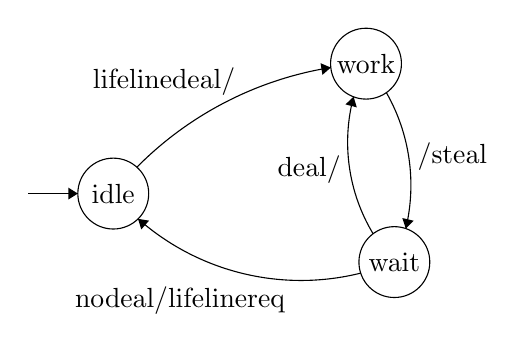
\begin{tikzpicture}[scale=0.15]
\tikzstyle{every node}+=[inner sep=0pt]
\draw [black] (20.9,-23.3) circle (3);
\draw (20.9,-23.3) node {idle};
\draw [black] (42.3,-12.3) circle (3);
\draw (42.3,-12.3) node {work};
\draw [black] (44.7,-29.1) circle (3);
\draw (44.7,-29.1) node {wait};
\draw [black] (22.9,-21.066) arc (135.27934:99.12868:29.75);
\fill [black] (39.32,-12.63) -- (38.45,-12.26) -- (38.61,-13.25);
\draw (25.2,-15.02) node [above] {lifelinedeal/};
%\draw [black] (43.382,-9.514) arc (186.50322:-101.49678:2.25);
%\fill [black] (45.17,-11.46) -- (46.02,-11.87) -- (45.91,-10.88);
\draw [black] (44.023,-14.75) arc (29.69026:-13.43006:15.827);
\fill [black] (45.67,-26.27) -- (46.34,-25.6) -- (45.37,-25.37);
\draw (46.63,-20.18) node [right] {/steal};
\draw [black] (42.903,-26.704) arc (-148.86241:-194.87738:14.991);
\fill [black] (41.25,-15.1) -- (40.56,-15.75) -- (41.52,-16);
\draw (40.2,-21.24) node [left] {deal/};
\draw [black] (41.852,-30.034) arc (-75.95772:-131.43403:20.846);
\fill [black] (23,-25.44) -- (23.27,-26.34) -- (23.93,-25.59);
\draw (26.55,-31.11) node [below] {nodeal/lifelinereq};
\draw [black] (13.7,-23.3) -- (17.9,-23.3);
\fill [black] (17.9,-23.3) -- (17.1,-22.8) -- (17.1,-23.8);
\end{tikzpicture}
\caption{State diagram for UTS workers.\label{fig:uts-state}}
\end{figure}

TODO

Common implementation of WorkList. Show interface. Explain mutability and
ownership are for performance.

Akka: implementation using vanilla actors (no akka-fsm). Work is split up by
sending \lstinline{Work} messages to oneself. State transitions are implemented
using \lstinline{become}.

Termination is difficult.

UTS: three problems, three solutions.

UTS \apgas: concurrency control implemented as multiple paradigms (synchronized
data access, global invariants, active messages). Concurrency is more
fine-grained.
